% Chapter Template

\chapter{BDI ( Belief-Desire-Intention)} % Main chapter title

\label{Chapter4} % Change X to a consecutive number; for referencing this chapter elsewhere, use \ref{ChapterX}

%----------------------------------------------------------------------------------------
%	SECTION 1
%----------------------------------------------------------------------------------------

Les agents de BDI sont basés sur les concepts philosophiques d'intentions, de plans et de raisonnements pratiques développés par Bratman \parencite{bratman1987intention}. Ce modèle est basé sur la psychologie populaire, c'est-à-dire la manière dont nous pensons. Le modèle fournit une première approximation de la cognition humaine, mais il reste encore beaucoup à faire pour l’affiner.


\section{Belief}

Les croyances d'un agent sont sa vision du monde, qui n'est pas nécessairement la même chose que l'état du monde, car les capteurs peuvent être imparfaits, en effet les informations fournies peuvent être à la fois incomplètes et bruyantes.

\section{Desire}

Plutôt que les désirs d’un agent, nous nous référons à ses objectifs. Ceux-ci donnent l'état du monde dans lequel l'agent souhaite être et doit être cohérent.


\section{Intention}

Ses intentions sont les plans qu'il exécute actuellement. Il peut y avoir plus d'un plan en cours, car un agent peut travailler simultanément à plusieurs objectifs (non conflictuels). Une fois qu'un agent a formulé une intention (c.-à-d. Qu'il sélectionne un plan), il est en quelque sorte engagé dans ce plan - il continue de l'exécuter (ou du moins a l'intention de l'exécuter) jusqu'à ce que l'objectif soit atteint, ou qu’il devienne impossible à atteindre en suivant ce même plan, l'objectif devient alors inutile. 
Un plan est une «recette» pour atteindre un objectif particulier. C'est une séquence d'actions et / ou de sous objectifs à réaliser. Si une étape de la séquence échoue, le plan lui-même échouera. L'une des caractéristiques d'un système BDI est que, lorsqu'un plan échoue, l'agent réessaye (si possible). Il tentera de trouver un autre moyen d’atteindre l’objectif en tenant compte du fait que le monde (et donc les convictions de l’agent ou son Desire) est en train de changer. Un agent stocke ses plans dans une bibliothèque de plans.


\section{Agent BDI}

L'agent montré à la Figure \ref{fig:bdi}, Page \pageref{fig:bdi} passe par un cycle continu de:

\begin{enumerate}
\item Ressentir l'environnement.
\item Raisonner sur les croyances, les objectifs et les intentions.
\item Accomplir une ou plusieurs actions.
\end{enumerate}

Ce cycle est très similaire à celui utilisé dans SWARMM section \ref{ssec:swarm}, qui sépare la deuxième étape en deux étapes: évaluation de la situation suivie de la sélection tactique. En effet, SWARMM est implémenté en utilisant une architecture BDI. Au cours de la phase de raisonnement du cycle, l'agent doit raisonner sur les croyances (si et comment elles devraient changer), les objectifs (les changements de croyances peuvent affecter la faisabilité des objectifs) et les intentions (les changements d'objectifs peuvent amener l'agent à abandonner certaines intentions et / ou d’en créer de nouvelles ). L'agent doit également décider quelle action (ou quelles actions) effectuer ensuite, à partir des intentions actuelles.


\begin{figure}[th]
\centering
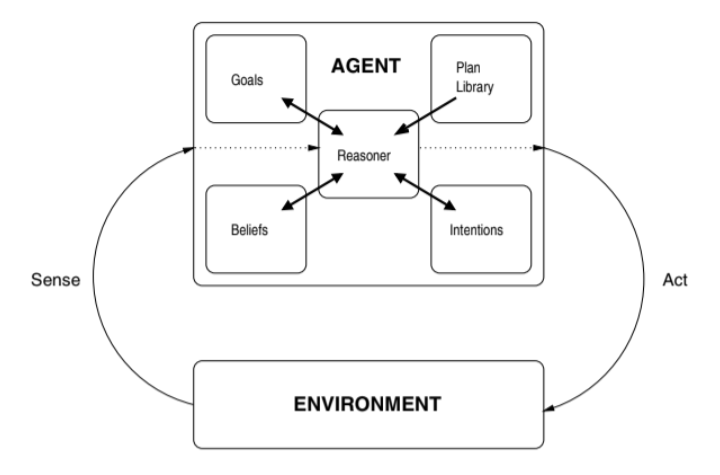
\includegraphics{Figures/bdi.PNG}
\decoRule
\caption[ Structure d’un agent BDI ] { Structure d’un agent BDI }
\label{fig:bdi}
\end{figure}


~\par
Lorsqu'il existe plusieurs plans disponibles pour atteindre un objectif donné, l'agent utilise en théorie un choix rationnel pour sélectionner un plan \parencite{bratman1988plans}. C'est-à-dire que les avantages de tous les plans applicables sont évalués et que le «meilleur» est sélectionné. Cependant la recherche en NDM indique que ce n'est pas ainsi que les gens prennent leurs décisions, et c'est sur cela que le travail doit être fait pour  améliorer le modèle BDI .

~\par
Dans les implémentations pratiques d'architectures BDI, telles que JACK \parencite{jack} ou dMARS \parencite{dmars1997formal}, chaque plan est conçu pour gérer un objectif particulier dans un contexte particulier. (Dans ces systèmes, le "contexte" est un ensemble de conditions que l'agent doit croire vraies.) Cela permet au programmeur de spécifier différentes manières d'atteindre le même objectif dans différentes situations, mais il est également possible d'avoir plusieurs plans applicables dans une situation donnée (lorsque les contextes se chevauchent).
